\documentclass[CJKutf8,xcolor=pdftex,dvipsnames,table]{beamer}
\usepackage{hyperref}
\hypersetup{
  pdftitle={Operating System Concepts},
  pdfauthor={Hong MingJian},
  pdfsubject={Process Management},
  pdfpagemode={FullScreen},
  colorlinks={true},
  linkcolor={blue},
}
\usepackage{CJKutf8}
\usepackage{epic} % for \dashline
\usepackage{listings}
\lstset{
	language=[ANSI]C,
	basicstyle=\scriptsize,
	tabsize=2,
	breaklines=true,
	keywordstyle=\color{blue},
	identifierstyle=,
	commentstyle=\color{OliveGreen},
	stringstyle=,
	showstringspaces=false,
  extendedchars=false
%  numbers=left,
%  numberstyle=\tiny
}

\usetheme{Madrid}%{Warsaw}
\usecolortheme{crane}

\begin{document}
\begin{CJK*}{UTF8}{song}

  \title{\CJKfamily{hei} 操作系统原理}
  \subtitle{\CJKfamily{hei} 第四章:进程管理}
	\author{\CJKfamily{hei} 洪明坚}
	\institute{\CJKfamily{hei} 重庆大学软件学院}
  \date{\today}

  \AtBeginSection[]
  {
    \begin{frame}
      \frametitle{Outline}
      \tableofcontents[currentsection]
    \end{frame}
  }

  \frame{\titlepage}

  \frame{\frametitle{目录}\tableofcontents}

  \section{Process}
  
  %% PAGE
  \begin{frame}
  \frametitle{Process concept (1/3)} \pause
  \begin{itemize}
  \item{Before the advent of process} \pause
    \begin{itemize}
    \item{Batch system \pause - \textbf{job};} \pause
    \item{Multiprogramming or time-sharing \pause - \textbf{program or task}.} \pause
    \end{itemize}
  \item{\textbf{Process}} \pause
    \begin{itemize}
    \item{\textbf{An abstraction of a running job/program/task}.}
    \end{itemize}
  \end{itemize}
  \end{frame}

  %% PAGE
  \begin{frame}
  \frametitle{Process concept (2/3)} \pause
  \begin{itemize}
  \item{What's a process?} \pause
    \begin{itemize}
    \item{A program in execution.} \pause
    \end{itemize}
  \item{A process is MUCH more than a program. It consists of} \pause
    \begin{itemize}
    \item{\textbf{Text section} (executable machine codes) from the program file;} \pause
    \item{\textbf{Data section} (the global variables) from the program file;} \pause
    \item{\emph{Contents} of the processor's \textbf{registers};} \pause
    \item{\textbf{Stack} which contains temporary data such as function parameters, return addresses and local variables;} \pause
    \item{\textbf{Heap} which is the memory used to be allocated dynamically if necessary;} \pause
    \item{A lot of other resources such as open files, etc.}
    \end{itemize}
  \end{itemize}
  \end{frame}

  %% PAGE
  \begin{frame}
  \frametitle{Process concept (3/3)} \pause
  \begin{itemize}
  \item{\textbf{Process image} in memory} \pause
  \end{itemize}
  \begin{center}
    \includegraphics[scale=0.5]{pi}
  \end{center}
  \end{frame}

  \subsection{Process and Program}

  %% PAGE
  \begin{frame}
  \frametitle{Program v.s. process} \pause
  \begin{itemize}
  \item{The program is a \textbf{passive} entity which resides in some storage;} \pause
    \begin{itemize}
    \item{While the process is an \textbf{active} entity which contains a lot of resources other than the program.} \pause
    \end{itemize}
  \item{Many processes may be running the same program. But,} \pause
    \begin{itemize}
    \item{They are considered as separate execution sequences although they share the same text section;} \pause
    \item{Other resources usually vary.}
    \end{itemize}
  \end{itemize}
  \end{frame}

  \subsection{Process state}

  %% PAGE
  \begin{frame}
  \frametitle{Process state} \pause
  \begin{itemize}
  \item{As a process executes, it changes \textbf{state}.} \pause
    \begin{itemize}
    \item{The state of the process is defined by its current activity.} \pause
    \end{itemize}
  \item{Each process may be in one of the following states:} \pause
    \begin{itemize}
    \item{\textbf{New} \pause - The process is being created;} \pause
    \item{\textbf{Running} \pause - Instructions are being executed;} \pause
    \item{\textbf{Waiting} \pause - The process is waiting for some event to occur;} \pause
    \item{\textbf{Ready} \pause - The process is waiting to be assigned to a processor;} \pause
    \item{\textbf{Terminated} \pause - The process has finished its execution.}
    \end{itemize}
  \end{itemize}
  \end{frame}

  %% PAGE
  \begin{frame}
  \frametitle{State transition (1/2)} \pause
  \begin{itemize}
  \item{As the process proceeds, it will transit from current state to another.}
    \begin{itemize}
    \item{There are six transitions among these five states.} \pause
    \end{itemize}
  \end{itemize}
  \begin{center}
    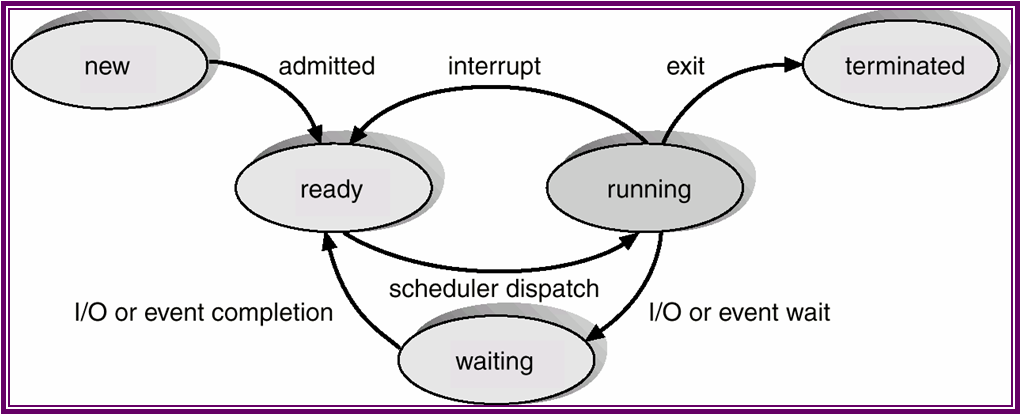
\includegraphics[scale=0.5]{v6f4-1}
  \end{center}
  \end{frame}

  %% PAGE
  \begin{frame}
  \frametitle{State transition (2/2)} \pause
  \begin{itemize}
  \item{Transitions} \pause
    \begin{description}
    \item[Admitted]{The process has been created and is ready to run;} \pause
    \item[Scheduler dispatch]{The \textbf{scheduler} picks the process to run;} \pause
    \item[Interrupt]{An interrupt has occurred;} \pause
    \item[I/O event wait]{The process blocks for I/O completion or reception of an signal;} \pause
    \item[I/O event completion]{I/O has completed or an event has occurred;} \pause
    \item[Exit]{The process has finished its execution.}
    \end{description}
  \end{itemize}
  \end{frame}

  \subsection{Process control block}

  %% PAGE
  \begin{frame}
  \frametitle{Process Control Block} \pause
  \begin{minipage}[c]{0.6\textwidth}
    \begin{itemize}
    \item{Each process is represented in the operating system by a \textbf{Process Control Block (PCB)}.} \pause
      \begin{itemize}
      \item{Also known as \textbf{Task Control Block}.} \pause
      \end{itemize}
    \item{Notes} \pause
      \begin{enumerate}
      \item{\textbf{Process number} is an unique identifier of a process, also known as \textbf{PID}.} \pause
      \item{\textbf{Program counter (PC)} is one of registers.} \pause
      \item{\textbf{Scheduling information} includes process' priority, etc.} \pause
      \end{enumerate}
    \end{itemize}
  \end{minipage}%
  \begin{minipage}[c]{0.4\textwidth}
    \centering
    \includegraphics[scale=0.6]{pcb}
  \end{minipage}
  \end{frame}

  %% PAGE
  \begin{frame}
  \frametitle{Questions}
  \begin{itemize}
  \item{Any questions?}
  \end{itemize}
  \begin{center}
    
\includegraphics[scale=.5]{question}
  \end{center}
  \end{frame}

  \section{Process scheduling}

  %% PAGE
  \begin{frame}
  \frametitle{Process scheduling} \pause
  \begin{itemize}
  \item{When running process can not proceed for some reason, the operating system must \textbf{decide which process to run next}.} \pause
    \begin{itemize}
    \item{Three main concerns:} \pause
      \begin{enumerate}
      \item{What happens to the process currently running?} \pause
      \item{How to keep track of what each process should be doing?} \pause
      \item{How to decide which process to run next?}
      \end{enumerate}
    \end{itemize}
  \end{itemize}
  \end{frame}

  \subsection{Context switch}

  %% PAGE
  \begin{frame}
  \frametitle{Concern 1} \pause
	  \begin{itemize}
	  \item{What happens to the process currently running?} \pause
	    \begin{itemize}
	    \item{\textbf{Context switch}} \pause
	    \end{itemize}
	  \end{itemize}
  \setlength{\unitlength}{0.6cm}
  \begin{picture}(20, 14)
    \put(1, 6.5){\includegraphics[scale=0.3]{pcb}}
    \put(1.2, 5.7){$PCB_A$}
    \put(17, 6.5){\includegraphics[scale=0.3]{pcb}}
    \put(17.2, 5.7){$PCB_B$}
    \pause
    \put(7.5, 14){\vector(0, -1){1}}
    \put(7.5, 13.2){\color{red}A running\color{black}}
    \pause
    \put(5.8, 12.5){save context}
    \dashline{0.2}(5.8, 12.5)(3.8, 11.9)
    \dashline{0.2}(5.8, 12.5)(3.8, 6.5)
    \pause
    \put(7.5, 12.5){\line(0, -1){1}}
    \put(7.5, 11.5){\line(1, 0){5}}
    \put(8.5, 11.3){schedule}
    \put(12.5, 11.5){\vector(0, -1){1}}
    \pause
    \put(9.9, 10){restore context}
    \dashline{0.2}(14.5, 10)(17, 11.9)
    \dashline{0.2}(14.5, 10)(17, 6.5)
    \pause
    \put(12.5, 10){\vector(0, -1){2}}
    \put(8.8, 8.8){\color{red}B running\color{black}}
    \pause
    \put(10.8, 7.7){save context}
    \dashline{0.2}(14.5, 7.7)(17, 11.9)
    \dashline{0.2}(14.5, 7.7)(17, 6.5)
    \pause
    \put(12.5, 7.7){\line(0, -1){1}}
    \put(12.5, 6.7){\line(-1, 0){5}}
    \put(8.5, 6.5){schedule}
    \put(7.5, 6.7){\vector(0, -1){1}}
    \pause
    \put(4.9, 5.2){restore context}
    \dashline{0.2}(4.9, 5.2)(3.8, 11.9)
    \dashline{0.2}(4.9, 5.2)(3.8, 6.5)
    \pause
    \put(7.5, 5.2){\vector(0, -1){1}}
    \put(7.5, 4.4){\color{red}A running\color{black}}
  \end{picture}
  \end{frame}

   %% PAGE
%  \begin{frame}
%  \frametitle{Context switch (1/2)} \pause
%  \begin{center}
%    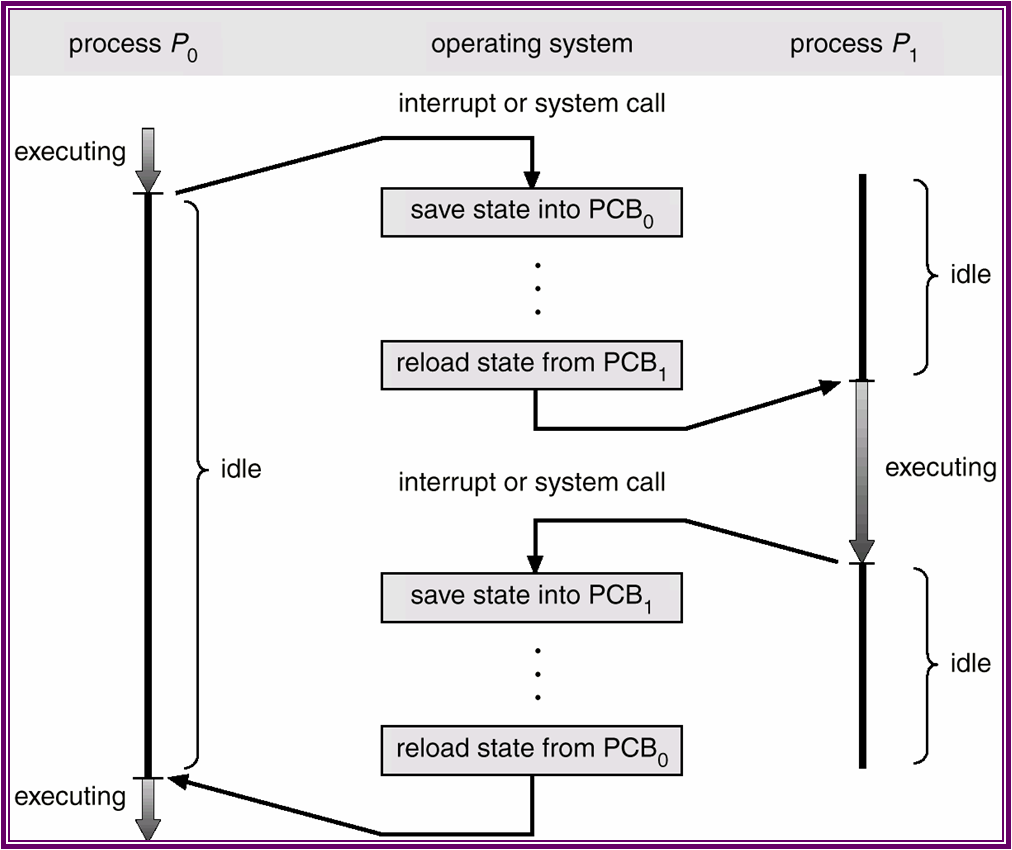
\includegraphics[scale=0.5]{v6f4-3}
%  \end{center}
%  \end{frame}

  %% PAGE
  \begin{frame}
  \frametitle{Context switch} \pause
  \begin{itemize}
  \item{Context switch is \textbf{pure} overhead.} \pause
    \begin{itemize}
    \item{Depending on the underling processor, it may burn \textbf{a lot of} CPU cycles.} \pause
    \item{Context switching has become such as performance bottleneck that programmers are using a new structure to avoid it whenever possible.}
    \end{itemize}
  \end{itemize}
  \end{frame}

  \subsection{Scheduling queues}

  %% PAGE
  \begin{frame}
  \frametitle{Concern 2} \pause
  \begin{itemize}
  \item{How to keep track of what each process should be doing?} \pause
    \begin{itemize}
    \item{\textbf{Scheduling queues}} \pause
      \begin{itemize}
      \item{\textbf{Job queue} \pause - consists of all processes in the system;} \pause
      \item{\textbf{Ready queue} \pause - consists of processes waiting for CPU to execute;} \pause
      \end{itemize}
    \item{The operating system also has other queues.} \pause
      \begin{itemize}
      \item{\textbf{I/O device queue} \pause - consists of processes waiting for a particular I/O device.}
      \end{itemize}
    \end{itemize}
  \end{itemize}
  \end{frame}

  %% PAGE
  \begin{frame}
  \frametitle{Various I/O device queues} \pause
  \begin{center}
  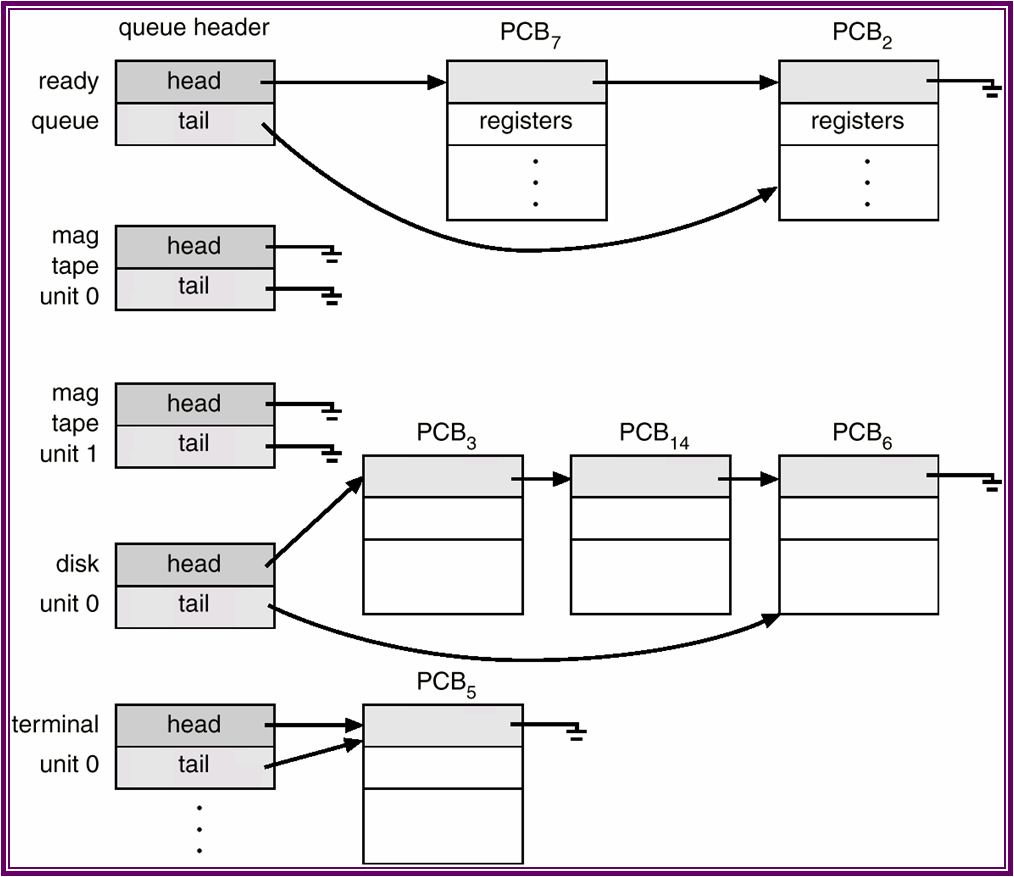
\includegraphics[scale=0.5]{v6f4-4}
  \end{center}
  \end{frame}

  %% PAGE
  \begin{frame}
  \frametitle{Queuing diagram} \pause
  \begin{itemize}
  \item{The queuing diagram is a common representation of process scheduling in the operating system.} \pause
  \end{itemize}
  \begin{center}
  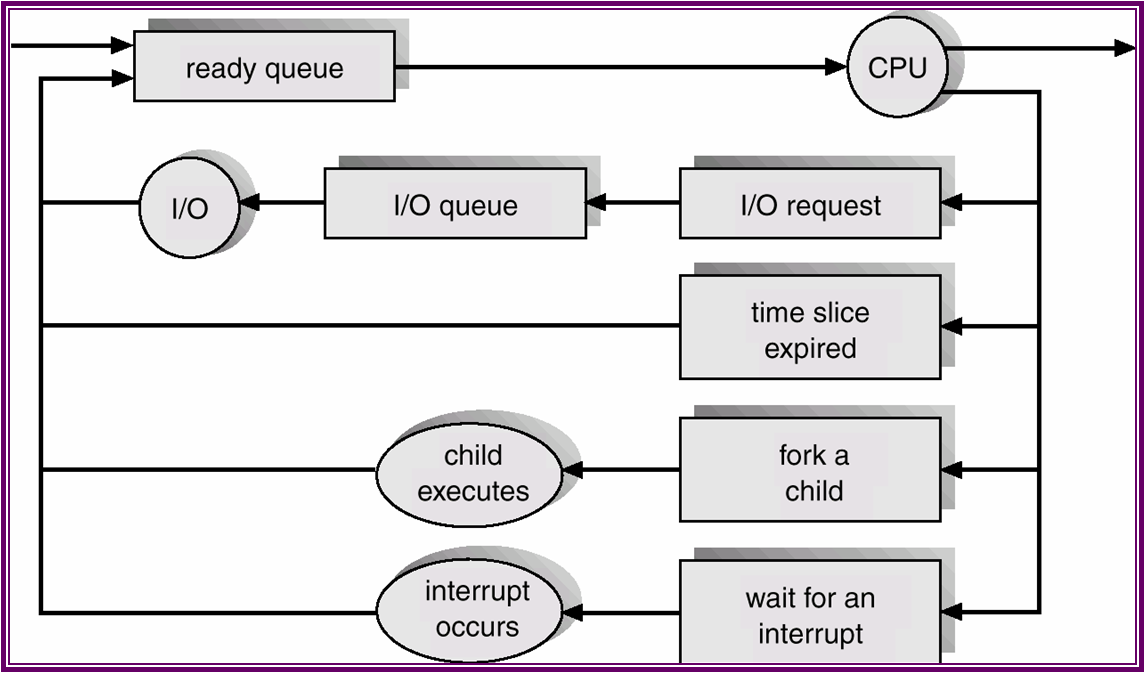
\includegraphics[scale=0.4]{v6f4-5}
  \end{center}
  \end{frame}

  \subsection{The scheduler}
  
  %% PAGE
  \begin{frame}
  \frametitle{Concern 3} \pause
  \begin{itemize}
  \item{How to decide which process to run next?} \pause
    \begin{itemize}
    \item{It's the \textbf{scheduler} which makes this decision.} \pause
    \end{itemize}
  \item{The scheduler selects a process from the ready queue and allocates CPU to it.} \pause
    \begin{itemize}
    \item{We call this scheduler the \textbf{CPU scheduler}.}
    \end{itemize}
  \end{itemize}
  \end{frame}

\iffalse

  %% PAGE
  \begin{frame}
  \frametitle{Schedulers (1/3)} \pause
  \begin{itemize}
  \item{\textbf{The CPU scheduler} (also known as \textbf{the short-term scheduler})} \pause
    \begin{description}
    \item[Operation:]{Allocates CPU to ready processes} \pause
    \item[Frequency:]{Frequent, about 100 ms one time} \pause
    \item[Objective:]{Ensure good response times in time-sharing systems} \pause
    \end{description}
  \item{\textbf{The admission scheduler} (also known as \textbf{the long-term scheduler})} \pause
    \begin{description}
    \item[Operation:]{Creates processes and adds them to the ready queue} \pause
    \item[Frequency:]{Infrequent, about one or several minutes} \pause
    \item[Objective:]{Maintain good throughput by controlling \textbf{the degree of multiprogramming} and ensuring mix of \textbf{I/O- and CPU-bound} processes}
    \end{description}
  \end{itemize}
  \end{frame}

  %% PAGE
  \begin{frame}
  \frametitle{Schedulers (2/3)} \pause
  \begin{itemize}
  \item{\textbf{The memory scheduler} (also known as \textbf{the medium-term scheduler})} \pause
    \begin{description}
    \item[Operation:]{Bring the processes in or out of the memory according to the available memory} \pause
    \item[Frequency:]{Between the short- and long-term schedulers} \pause
    \item[Objective:]{Reduce the degree of multiprogramming when the long-term scheduler underestimates process requirements} \pause
    \end{description}
    \begin{center}
      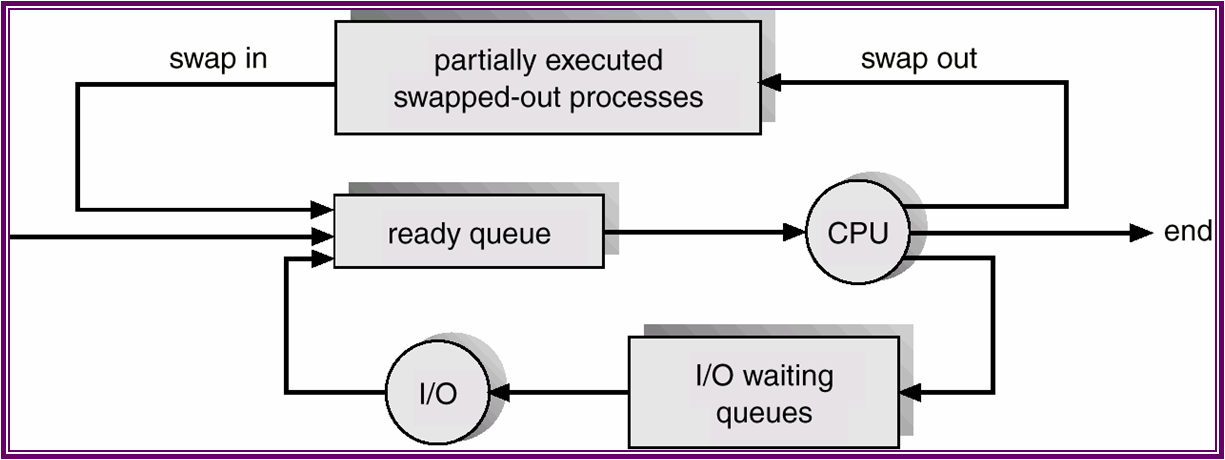
\includegraphics[scale=0.4]{v6f4-6}
    \end{center}
  \end{itemize}

  \end{frame}

  %% PAGE
  \begin{frame}
  \frametitle{Schedulers (3/3)} \pause
  \begin{center}
    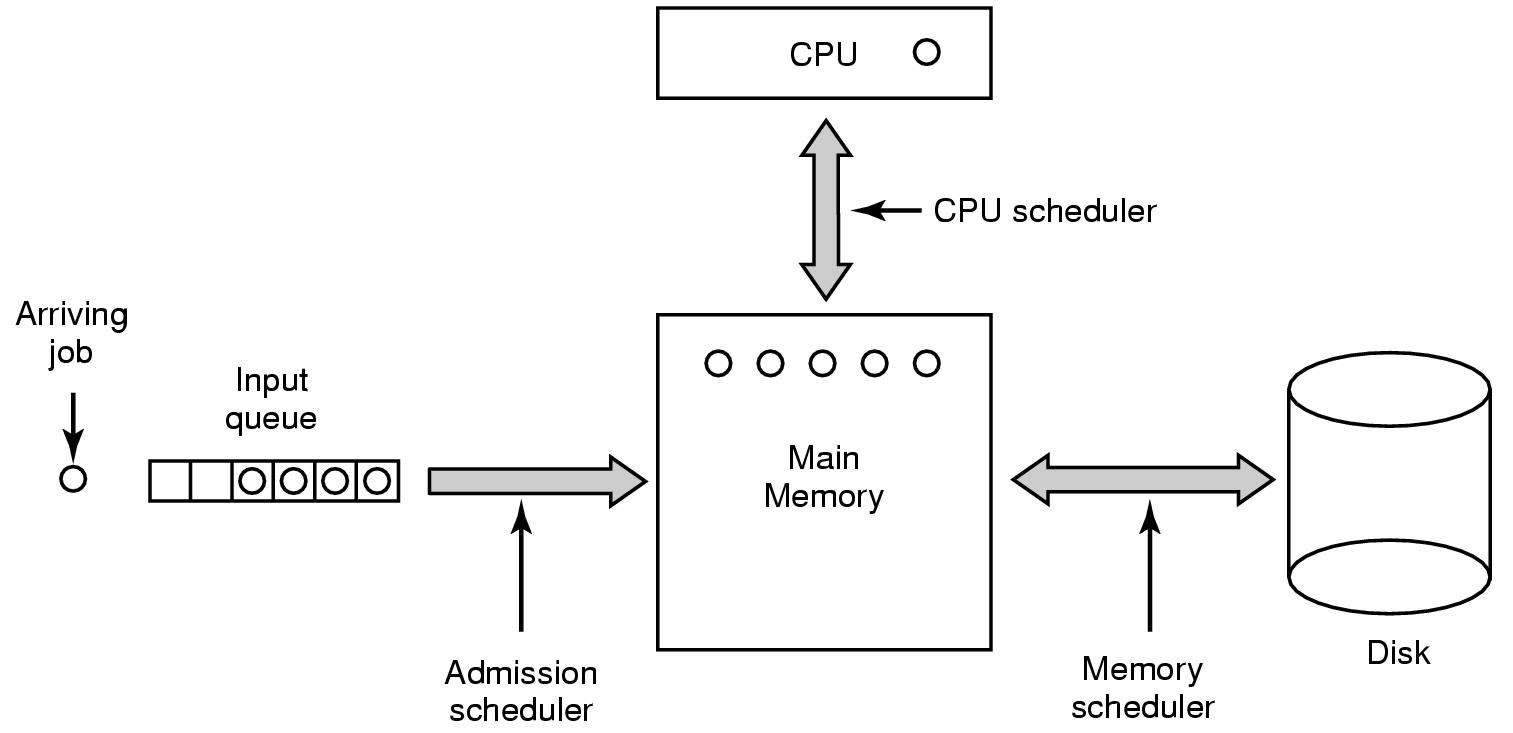
\includegraphics[scale=0.2]{mosv2f2-40} \pause
  \end{center}
  \begin{itemize}
  \item{The schedulers depend on the \textbf{scheduling algorithms} to make the decision.} \pause
    \begin{itemize}
    \item{We will return to scheduling algorithm later.}
    \end{itemize}
  \end{itemize}
  \end{frame}
  
\fi

  %% PAGE
  \begin{frame}
  \frametitle{Questions}
  \begin{itemize}
  \item{Any questions?}
  \end{itemize}
  \begin{center}
    
\includegraphics[scale=.5]{question}
  \end{center}
  \end{frame}

  \section{Operations on process}

  \subsection{Creation}
  
  %% PAGE
  \begin{frame}[fragile]
  \frametitle{Operations on process (1/2)} \pause
  \begin{itemize}
  \item{Creation \pause - a ``parent'' process spawns a ``child'' process.} \pause
    \begin{itemize}
    \item{Parent process create children processes, which, in turn create other processes, forming a tree of processes.} \pause
    \item{For example, \emph{fork} in Linux/Unix and \emph{CreateProcess} in Windows.} \pause
    \end{itemize}
  \end{itemize}
\begin{lstlisting}
          int main() {
            int pid = fork(); /*fork another process*/
            if(pid < 0) {     /*error occurred*/
              printf("fork failed\n");
              exit(-1);
            } else if (pid == 0) /*in child process*/
              execlp("/bin/ls", "ls", NULL); /*executes a program*/
            else { /*in parent process*/
              waitpid(pid,NULL,0); /*waiting for the child to exit*/
              printf("Child exited\n");
              exit(0);
            }
          }
\end{lstlisting}
	\end{frame}

  \subsection{Termination}

  %% PAGE
  \begin{frame}
  \frametitle{Operations on process (2/2)} \pause
  \begin{itemize}
  \item{Termination. \pause Two kinds of termination:} \pause
    \begin{description}
    \item[normal]{a process asks the operating system to delete it. For example, \emph{exit} in Linux/Unix and \emph{ExitProcess} in Windows.} \pause
    \item[abnormal]{one process may be killed by another process by \emph{kill} in Linux/Unix and \emph{TerminateProcess} in Windows.} \pause
    \end{description}
  \item{Communication \pause - facilities used by one process to communicate with another.} \pause
  \item{Cooperation \pause - cooperating processes need to synchronize their actions.}
  \end{itemize}
  \end{frame}

  %% PAGE
  \begin{frame}
  \frametitle{Questions}
  \begin{itemize}
  \item{Any questions?}
  \end{itemize}
  \begin{center}
    
\includegraphics[scale=.5]{question}
  \end{center}
  \end{frame}

  \section{Cooperating processes}

  %% PAGE
  \begin{frame}
  \frametitle{Cooperating processes} \pause
  \begin{itemize}
  \item{A process can be} \pause
    \begin{itemize}
    \item{\textbf{independent} if it cannot affect or be affected by the other processes;} \pause
    \item{\textbf{cooperating} otherwise.} \pause
    \end{itemize}
  \item{There are several advantages for the process cooperation.} \pause
    \begin{description}
    \item[Information sharing:]{Several processes may be interested in the same piece of information;} \pause
    \item[Computation speedup:]{Break the problem into several subtasks that can be run in parallel;} \pause
    \item[Modularity:]{Separate processes for different functions by design;} \pause
%    \item[Convenience]{} \pause
    \end{description}
  \item{However, concurrent execution of cooperating processes requires mechanisms that allow processes to communicated with one another and to synchronize their actions.}
  \end{itemize}
  \end{frame}

  \subsection{The producer and consumer}

  %% PAGE
  \begin{frame}
  \frametitle{Example} \pause
  \begin{itemize}
  \item{\textbf{The producer and consumer problem}} \pause
    \begin{itemize}
    \item{A \textbf{producer} process produces information that is consumed by a \textbf{consumer} process.} \pause
    \item{This problem is a common paradigm for cooperating system.} \pause
    \end{itemize}
  \item{To allow producer and consumer processes to run concurrently, we need} \pause
    \begin{itemize}
    \item{a buffer which can be filled by the producer and emptied by the consumer;} \pause
    \item{to synchronize the producer and consumer.} \pause
    \end{itemize}
  \item{According the size of the buffer, we have} \pause
    \begin{itemize}
    \item{\textbf{unbounded-buffer} producer and consumer problem;} \pause
    \item{\textbf{bounded-buffer} producer and consumer problem.}
    \end{itemize}
  \end{itemize}
  \end{frame}

\iffalse

  %% PAGE
  \begin{frame}
  \frametitle{The bounded-buffer producer and consumer problem} \pause
  \begin{itemize}
  \item{The buffer can be provided by the operating system through the use of an \textbf{interprocess communication (IPC)} facility.} \pause
    \begin{itemize}
    \item{The programmers just use the system calls to fill or empty the buffer.} \pause
    \end{itemize}
  \item{The buffer can also be in a piece of shared memory which is accessible to both the producer and consumer.} \pause
    \begin{itemize}
    \item{In this case, the programmer must manage the shared buffer themselves.}
    \end{itemize}
  \end{itemize}
  \end{frame}

\fi

  %% PAGE
  \begin{frame}[fragile]
  \frametitle{Implementation} \pause
  \begin{itemize}
  \item{A solution to \textbf{bounded-buffer producer and consumer problem}.} \pause
  \end{itemize}
\begin{lstlisting}
                   /* Shared variables */
                   #define BSIZE 10
                   struct item {
                      ....
                   } buffer[BSIZE];
                   int in = 0, out = 0;
/*---------------------------------------------------------------*/
/*The producer loop*/                 /*The consumer loop*/
while(1) {                            while(1) {
  /*produce an item*/                   while(in == out)
  while(((in + 1) % BSIZE) == out)        /*do nothing*/;
      /*do nothing*/;                   itemConsumed = buffer[out];
  buffer[in] = itemProduced;            out = (out + 1) % BSIZE;
  in = (in + 1) % BSIZE;                /*consume the item*/
}                                     }
\end{lstlisting}
\end{frame}

  %% PAGE
  \begin{frame}
  \frametitle{Questions}
  \begin{itemize}
  \item{Any questions?}
  \end{itemize}
  \begin{center}
    
\includegraphics[scale=.5]{question}
  \end{center}
  \end{frame}

  \section{Interprocess communication (IPC)}

  %% PAGE
  \begin{frame}
  \frametitle{Interprocess communication (IPC)} \pause
  \begin{itemize}
%  \item{In the producer and consumer problem, we say that the buffer can be provided by the operating system.} \pause
%    \begin{itemize}
%    \item{The operating system must synchronize the access of producer and consumer to the buffer.} \pause
%    \end{itemize}
  \item{What's the IPC?} \pause
    \begin{itemize}
    \item{\textbf{IPC provides a mechanism to allow processes to communicate and to synchronize their actions without sharing the same address space}.} \pause
    \end{itemize}
  \item{Examples} \pause
    \begin{itemize}
    \item{Message-passing, pipe, socket, etc.} \pause
%    \item{We will focus on the message-passing here.}
    \end{itemize}
  \end{itemize}
  \end{frame}

  \iffalse

  \subsection{Message-passing}

  %% PAGE
  \begin{frame}
  \frametitle{Message-passing} \pause
  \begin{itemize}
  \item{Two operations:} \pause
    \begin{itemize}
    \item{\emph{send} \pause - send a message to someone} \pause
    \item{\emph{receive} \pause - receive a message from someone} \pause
    \end{itemize}
  \item{Implementation problems} \pause
    \begin{enumerate}
    \item{How are links established?} \pause
    \item{Can a link be associated with more than two processes?} \pause
    \item{How many links can there be between every pair of communicating processes?} \pause
    \item{What is the capacity of a link?} \pause
    \item{Is the size of a message that the link can accommodate fixed or variable?} \pause
    \item{Is a link unidirectional or bi-directional?}
    \end{enumerate}
  \end{itemize}
  \end{frame}

  %% PAGE
  \begin{frame}
  \frametitle{Direct communication} \pause
  \begin{itemize}
  \item{Processes must name each other explicitly:} \pause
    \begin{itemize}
    \item{\emph{send (P, message)} \pause - send a message to process P} \pause
    \item{\emph{receive(Q, message)} \pause - receive a message from process Q} \pause
    \end{itemize}
  \item{Properties of communication link} \pause
    \begin{itemize}
    \item{Links are established automatically.} \pause
    \item{A link is associated with exactly one pair of communicating processes.} \pause
    \item{Between each pair there exists exactly one link.} \pause
    \item{The link may be unidirectional, but is usually bi-directional.}
    \end{itemize}
  \end{itemize}
  \end{frame}

  %% PAGE
  \begin{frame}
  \frametitle{Indirect Communication (1/3)} \pause
  \begin{itemize}
  \item{Messages are directed and received from \textbf{mailboxes} (also referred to as \textbf{ports}).} \pause
    \begin{itemize}
    \item{Each mailbox has a unique id.} \pause
    \item{Processes can communicate only if they share a mailbox.} \pause
    \end{itemize}
  \item{Properties of communication link} \pause
    \begin{itemize}
    \item{Link established only if processes share a common mailbox} \pause
    \item{A link may be associated with many processes.} \pause
    \item{Each pair of processes may share several communication links.} \pause
    \item{Link may be unidirectional or bi-directional.}
    \end{itemize}
  \end{itemize}
  \end{frame}

  %% PAGE
  \begin{frame}
  \frametitle{Indirect Communication (2/3)} \pause
  \begin{itemize}
  \item{Operations} \pause
    \begin{itemize}
    \item{create a new mailbox} \pause
    \item{send and receive messages through mailbox} \pause
    \item{destroy a mailbox} \pause
    \item{\emph{send(A, message)} \pause - send a message to mailbox A} \pause
    \item{\emph{receive(A, message)} \pause - receive a message from mailbox A}
    \end{itemize}
  \end{itemize}
  \end{frame}

  %% PAGE
  \begin{frame}
  \frametitle{Indirect Communication (3/3)} \pause
  \begin{itemize}
  \item{Mailbox sharing} \pause
    \begin{itemize}
    \item{$P_1$, $P_2$, and $P_3$ share mailbox A.} \pause
    \item{$P_1$, sends; $P_2$ and $P_3$ receive.} \pause
    \item{Who gets the message?} \pause
    \end{itemize}
  \item{Solutions} \pause
    \begin{itemize}
    \item{Allow a link to be associated with at most two processes.} \pause
    \item{Allow only one process at a time to execute a receive operation.} \pause
    \item{Allow the system to select arbitrarily the receiver.  Sender is notified who the receiver was.}
    \end{itemize}
  \end{itemize}
  \end{frame}

  \subsection{Synchronization}

  %% PAGE
  \begin{frame}
  \frametitle{Synchronization} \pause
  \begin{itemize}
  \item{Message passing may be either blocking or non-blocking.} \pause
    \begin{itemize}
    \item{Blocking is considered synchronous} \pause
    \item{Non-blocking is considered asynchronous} \pause
    \end{itemize}
  \item{\emph{send} and \emph{receive} may be either blocking or non-blocking.}
  \end{itemize}
  \end{frame}

  %% PAGE
  \begin{frame}
  \frametitle{Buffering} \pause
  \begin{itemize}
  \item{Queue of messages attached to the link; implemented in one of three ways.} \pause
    \begin{enumerate}
    \item{Zero capacity (0 message) \pause - Sender must wait for receiver (\textbf{rendezvous}).} \pause
    \item{Bounded capacity (finite length of n messages) \pause - Sender must wait if link full.} \pause
    \item{Unbounded capacity (infinite length) \pause - Sender never waits.}
    \end{enumerate}
  \end{itemize}
  \end{frame}

  %% PAGE
  \begin{frame}
  \frametitle{Questions}
  \begin{itemize}
  \item{Any questions?}
  \end{itemize}
  \begin{center}
    
\includegraphics[scale=.5]{question}
  \end{center}
  \end{frame}

  \fi

  \subsection{Pipe}

  %% PAGE
  \begin{frame}
  \frametitle{Pipe (1/3)} \pause
  \begin{itemize}
  \item{\textbf{Pipe} \pause - a FIFO communication channel between two processes.} \pause
    \begin{itemize}
    \item{A pipe has two ends: one for reading from it and the other for writing to it.} \pause
    \end{itemize}
  \item{There are two kinds of pipe:} \pause
    \begin{itemize}
    \item{Anonymous pipe} \pause
      \begin{itemize}
      \item{An unnamed,simplex (one-way) channel used to transfer data between the parent and child processes.} \pause
      \item{It exists for as long as the process is running.} \pause
      \end{itemize}
    \item{Named pipe} \pause
      \begin{itemize}
      \item{As an extension of unnamed pipe, it can be simplex or full-duplex and may be used by any process to communicate with each other.} \pause
      \item{It can be permanent (as in Linux/Unix) or volatile (as in Windows).}
      \end{itemize}
    \end{itemize}
  \end{itemize}
  \end{frame}

  %% PAGE
  \begin{frame}[fragile]%[containsverbatim]
  \frametitle{Pipe (2/3)} \pause
\begin{lstlisting}
          int main() {
             int fd[2], pid;  char buf;
             
             if (pipe(fd) == -1) /* Create an anonymous pipe */
             { perror("pipe"); exit(-1); }
             if ((pid = fork()) < 0)
             { perror("fork"); exit(-1); }
             if (pid == 0) {     /* Child reads from pipe */
                 close(fd[1]);   /* Close unused write end */

                 while (read(fd[0], &buf, 1) > 0)
                     write(STDOUT_FILENO, &buf, 1);

                 close(fd[0]);
                 exit(0);
             } else {    /* Parent writes argv[1] to pipe */
                 close(fd[0]);   /* Close unused read end */
                 write(fd[1], "Hello, child!", 13);
                 close(fd[1]);   /* Reader will see EOF */
                 waitpid(pid,NULL,0);      /* Wait for child to exit*/
                 exit(0);
             }
          }
\end{lstlisting}
\end{frame}

  %% PAGE
  \begin{frame}
  \frametitle{Pipe (3/3)} \pause
  \centering
  \setlength{\unitlength}{0.6cm}
  \begin{picture}(20, 14)
    \put(1.5, 6){\framebox(5, 3){}}
    \put(3, 9.1){Parent}

    \pause

    \put(4.5, 8){fd[0]}
    \put(2, 6.5){fd[1]}

    \put(6.5, 3){\framebox(6, 0.8){anonymous pipe}}

    \put(1.5, 7){\line(-1, 0){1}}
    \put(0.5, 7){\line(0, -1){3.7}}
    \put(0.5, 3.3){\vector(1, 0){6}}

    \put(12.5, 3.3){\line(1, 0){1}}
    \put(13.5, 3.3){\line(-1, 1){5.2}}
    \put(8.3, 8.5){\vector(-1, 0){1.8}}

    \pause

    \put(7.5, 9.6){\vector(1, 0){4}}
    \put(9, 9.7){fork}

    \pause

    \put(12.5, 6){\framebox(5, 3){}}
    \put(14, 9.1){Child}

%    \pause

    \put(15.5, 8){fd[0]}
    \put(13, 6.5){fd[1]}

    \put(12.5, 7){\line(-1, 0){1}}
    \put(11.5, 7){\line(-2, -1){6.51}}
    \put(4.99, 3.7){\vector(1, 0){1.51}}

    \put(12.5, 3.7){\line(1, 0){6}}
    \put(18.5, 8.5){\line(0, -1){4.8}}
    \put(18.5, 8.5){\vector(-1, 0){1}}

    \pause

    \color{white}
    \thicklines

    \put(12.5, 3.3){\line(1, 0){1}}
    \put(13.5, 3.3){\line(-1, 1){5.2}}
    \put(8.3, 8.5){\vector(-1, 0){1.8}}

    \pause

    \put(12.5, 7){\line(-1, 0){1}}
    \put(11.5, 7){\line(-2, -1){6.51}}
    \put(4.99, 3.7){\vector(1, 0){1.51}}

    \thinlines
    \color{black}

    \pause

    \dashline{0.2}(0, 4.9)(20, 4.9)
    \put(19, 3){Kernel}
    \put(19, 6){User}

  \end{picture}
  \end{frame}

  %% PAGE
  \begin{frame}
  \frametitle{Questions}
  \begin{itemize}
  \item{Any questions?}
  \end{itemize}
  \begin{center}
    
\includegraphics[scale=.5]{question}
  \end{center}
  \end{frame}

  %% PAGE
\end{CJK*}
\end{document}
